\chapter{Increasing Your Value}

This chapter follows an original Jim Rohn lecture preserved in a curated playlist rather than in a formal course sequence. We keep close to the spoken order because the lecture is built as a chain: first a law of self-change, then a way to measure it, then a correction about value and time, then a ladder model of income, and only after that the autobiographical proof and the closing rule about working on oneself. Curation credit for the playlist belongs to LazyingArt LLC.

\section{Opening Formula and the Adventure of Personal Development}

The lecture begins with a rule that is simple enough to sound motivational, but it is really the governing relation for everything that follows:

\begin{equation}
\text{Everything changes for you} \Longleftarrow \text{You change}.
\end{equation}

Rohn immediately explains the direction of the arrow. We do not first change what is outside. We change what is inside. That is why the next sentence tightens the same claim into a more economic-looking form:

\begin{equation}
\text{Have More} \Longleftarrow \text{Become More}.
\end{equation}

This is not yet about wages or markets. It is the lecture's master variable. We are being told that outward result is downstream of inner development. Hence the sequence of admonitions: do not wish it were easier; wish you were better. Do not wish for fewer problems; wish for more skills. What is being introduced here is not optimism in the thin sense, but a causal shift from environment to person.

Rohn then names the theme directly: personal development. He frames it as an ongoing adventure that began for him at age twenty-five and has not stopped. That biographical remark matters because it keeps the formula from turning into a slogan carved in stone. The chapter should preserve the feeling that this rule is something one keeps discovering again by practice.

The transition to economics is then carefully motivated. If we want to help people understand personal development concretely, where do we begin? Rohn's answer is practical: start with money, not because money is the whole of life, but because money is easy to count.

\section{Why Start with Money? Counting as a Diagnostic}

The lecture pauses here to justify its own method. Money is not the only value. In fact, Rohn explicitly says so. But money is countable, and that makes it useful as a first instrument. In this spirit, we may record the methodological rule as

\begin{equation}
\text{Money}=\text{a first countable diagnostic, not the whole of value}.
\end{equation}

That sentence should not be made harder than it is. The point is simply that economics gives us a place where changes are visible. If we want to know whether we have errors in judgment, lack of discipline, or failures of development, then counting is a reasonable beginning.

This is one of the lecture's quiet but important transitions. We move from a broad law of self-change to a narrow test case where the consequences of self-change may be tracked. Only now does the lecture narrow into its real mathematical hinge.

\section{Value, Time, and the Marketplace}

Rohn now states what he calls the key to understanding economics: we get paid for bringing value to the marketplace. He immediately glosses the word \emph{marketplace} by another word, \emph{reality}. That gloss is not decorative. It hardens the claim. The marketplace is where things are actually measured and rewarded.

\begin{equation}
\text{Marketplace}=\text{Reality}.
\end{equation}

\begin{figure}[h]
\centering

\includegraphics[width=.78\linewidth]{lecture_17_figure_02.png}
\caption{Flipchart contrasting value and time. The board words are only partly legible, but \emph{Value}, \emph{time}, and a likely gloss toward \emph{reality} are visible.}
\end{figure}

The flipchart is helpful here, not because it supplies a fully legible derivation, but because it preserves the board layout of the distinction. The large word is \emph{Value}; the smaller note is \emph{time}; and the lower parenthetical note appears to point toward \emph{reality}. This is enough to justify a clean reconstruction nearby.

\subsection{Question \& Answer}

\paragraph{Question.} Do we get paid for time or for value?

\paragraph{Answer.} We get paid for value. Time is required to bring value to the marketplace, but time itself is not what is being bought.

The lecture's correction may therefore be written as

\begin{align}
\text{Pay} &\neq \text{Time alone},\\
\text{Pay} &\propto \text{Value brought to the marketplace}.
\end{align}

Rohn is careful here. He does not deny that time matters. Indeed, the lecture explicitly says that it takes time to bring value to the marketplace. But he then refuses the common simplification that one is “making so much an hour” in a literal sense. If that were true, as he jokes, one could stay home and have the money sent over. The hour is the container; value is the content.

A compact way to keep the lecture's board logic visible is the following narrow schema:

\begin{figure}[h]
\centering
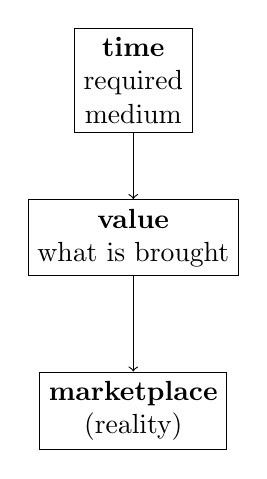
\begin{tikzpicture}
\node[draw, align=center] (t) at (0,2.8) {\textbf{time}\\required\\medium};
\node[draw, align=center] (v) at (0,0.8) {\textbf{value}\\what is brought};
\node[draw, align=center] (m) at (0,-1.4) {\textbf{marketplace}\\(reality)};
\draw[->] (t) -- (v);
\draw[->] (v) -- (m);
\end{tikzpicture}
\caption{Transcript-derived reconstruction of the lecture's value-time-marketplace relation.}
\end{figure}

The lecture then tightens its formulation one step further: we get paid for the value we put in the time. This is the sentence that prepares the next explicit puzzle.

\section{Multiplying Value in the Same Time}

Having corrected the variable, Rohn immediately asks what now becomes possible. If pay is for value, not time alone, then can we become twice as valuable and make twice as much money in the same time? Can we become three times as valuable and make three times as much in the same time?

\subsection{Question \& Answer}

\paragraph{Question.} Is it possible to make more money in the same time?

\paragraph{Answer.} Yes. If we can raise the value brought to the marketplace while holding time fixed, then pay can rise with it.

This is the lecture's cleanest worked implication, and we can make it explicit with very light notation. Let \(T\) denote time, \(V\) value, and \(P\) pay. The lecture's rule is not a textbook wage model; it is an operational relation. Holding \(T\) fixed, we have

\begin{align}
P &= kV,\\
V_2 = 2V_1 \quad &\Longrightarrow \quad P_2 = 2P_1,\\
V_3 = 3V_1 \quad &\Longrightarrow \quad P_3 = 3P_1.
\end{align}

The point is not the constant \(k\). The point is that the lecture now has a mathematically usable spine. Once time is held fixed, value becomes the variable that can move the result. Rohn's emphatic answer, “of course,” is not merely applause rhetoric. It is the lecture's endorsement of the implication

\begin{equation}
\text{Earn more money in the same time} \Longleftarrow \text{Become more valuable}.
\end{equation}

This section should preserve its logical force. The question is raised because the previous section made it raiseable. The answer matters because it then becomes the rule that governs everything after it.

\section{The Ladder: Starting Wage, Climbing, and High Income}

The lecture next changes register. We move from abstract relation to public picture. America, Rohn says, is a ladder to climb. It is not a bed. This metaphor does important work: it converts a question about starting wage into a question about motion.

\begin{equation}
\text{America is a ladder to climb}.
\end{equation}

\begin{figure}[h]
\centering

\includegraphics[width=.62\linewidth]{lecture_17_figure_03.png}
\caption{Flipchart wage example near \(\$4\) an hour. The writing is fragmentary, but the visible numeric mark supports the starting-rung discussion.}
\end{figure}

The board fragment is not a full ladder drawing, and we should not pretend otherwise. But it does preserve the numeric turn of the lecture: the discussion of a starting wage around \(\$4\) an hour and the neighboring debate that it “should be five.”

A cautious clean reconstruction is therefore

\begin{equation}
\text{Start at } \$4/\text{hour}.
\end{equation}

Rohn's answer to the political argument is revealing. It does not need to be five, because the point of a ladder is not to remain forever on the bottom rung. That lets him turn the issue from starting point to climbing rule:

\begin{equation}
\$4 \to \$5 \to \cdots
\end{equation}

\begin{figure}[h]
\centering
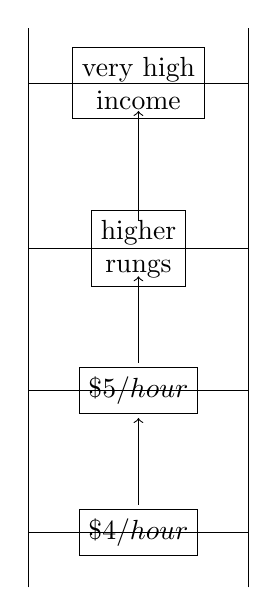
\begin{tikzpicture}
\node[draw, align=center] (r1) at (0,0) {\(\$4/\text{hour}\)};
\node[draw, align=center] (r2) at (0,1.8) {\(\$5/\text{hour}\)};
\node[draw, align=center] (r3) at (0,3.6) {higher\\rungs};
\node[draw, align=center] (r4) at (0,5.7) {very high\\income};
\draw ( -1.4,-0.7) -- (-1.4,6.4);
\draw ( 1.4,-0.7) -- ( 1.4,6.4);
\draw (-1.4,0.0) -- (1.4,0.0);
\draw (-1.4,1.8) -- (1.4,1.8);
\draw (-1.4,3.6) -- (1.4,3.6);
\draw (-1.4,5.7) -- (1.4,5.7);
\draw[->] (0,0.35) -- (0,1.45);
\draw[->] (0,2.15) -- (0,3.25);
\draw[->] (0,3.95) -- (0,5.35);
\end{tikzpicture}
\caption{Transcript-derived ladder reconstruction. The frames show the numeric example, while the ladder itself is reconstructed from the spoken lecture.}
\end{figure}

Here the lecture folds social metaphor back into causal law. The more valuable we become, the higher we move up the ladder. This is why the section widens so quickly from \(\$4\) per hour to the Disney executive earning fifty-two million dollars a year. Rohn's point is not that everyone will occupy the top rung. His point is that the ladder is not flat, and that value explains vertical motion.

\subsection{Question \& Answer}

\paragraph{Question.} How do we get more money?

\paragraph{Answer.} Not by treating the ladder as a bed, and not by fixing our whole attention on the bottom rung. We get more money by becoming more valuable and climbing.

The lecture sharpens this into a pair of relations:

\begin{align}
\text{Low marketplace value} &\Longrightarrow \text{Low marketplace pay},\\
\text{High marketplace value} &\Longrightarrow \text{High marketplace pay}.
\end{align}

\section{Marketplace Reality and False Strategies}

This is the hardest conceptual turn in the chapter because it is easy to state too crudely. Rohn says that someone may be valuable in many senses and still not be very valuable to the marketplace. One may be a valuable brother, a valuable member of the community, a valuable member of the church, valuable in the sight of God, valuable to the human family. But the marketplace measures a narrower thing.

The lecture's point is not that moral value and economic value are identical. It is precisely that they are distinct. That is why he repeats that the marketplace is called reality. In the register of pay, one is rewarded for marketplace value.

This distinction prepares the lecture's rejection of false causal strategies. Going on strike for more, demanding more, or simply waiting for a raise are treated as errors because they do not address the real variable. In the lecture's compressed logic,

\begin{equation}
\text{Demand} \not\Longrightarrow \text{Riches}.
\end{equation}

And in a more comparative form,

\begin{equation}
\text{Waiting for a raise} < \text{Climbing by added value}.
\end{equation}

This is also why the \(\$400\)-an-hour example appears later in the talk. The point of that example is not extravagance for its own sake. It is the same relation extended upward: the company pays that much because the person has become that valuable to the marketplace.

\section{Proof by Example: The Call Worth Millions}

The lecture now turns from structure to proof by example. Rohn tells the story of a phone call from a company ready to expand internationally, a call that would add millions to his fortune. At first the fact that they called him seems surprising. Then comes the decisive second thought: of course they would call him. Who else would they call if he could get the job done?

The story verifies the rule already established:

\begin{equation}
\text{Telephone call worth millions} \Longleftarrow \text{I had become valuable}.
\end{equation}

This is one of the lecture's most important recaps. The phone call is not a new principle. It is the old principle returned in narrative form. A farm boy from Idaho, one year of college, broke at twenty-five, creditors calling, pennies in pocket, nothing in the bank, promises behind. How can such a person later receive a call worth millions? The answer, repeated twice in the lecture, is simple: he changed.

The chapter should preserve that double movement. First the gap in circumstance, then the explanation by changed self. In this way the anecdote closes the loop back to the opening law of the lecture.

\section{Shoaff's Secret and the Return to the Inside}

The final section gives the lecture its distilled maxim. Shoaff's secret, Rohn says, was this: learn to work harder on yourself than you do on your job. Once he understood that, his life turned around.

The rule is given in two parallel implications:

\begin{align}
\text{Work hard on your job} &\Longrightarrow \text{Make a living},\\
\text{Work hard on yourself} &\Longrightarrow \text{Make a fortune}.
\end{align}

Here again we must hear the lecture carefully. “Fortune” does not finally remain only economic. The last movement of the talk expands self-work into a list: philosophy, attitude, personality, language, the gift of communication, all of one's abilities. This matters because the lecture ends by returning to the inside. Economics was the opening measurement, not the final horizon.

The last recurrence of the main rule may therefore be stated as

\begin{equation}
\text{Make yourself more valuable to the marketplace} \Longrightarrow \text{Change in income},
\end{equation}

but the lecture immediately broadens this into a more comprehensive formulation: when we work on the inside, promotions, money, economics, and future become easier because we are finally working on the right thing.

\section{Summary}

The lecture's mathematical core is narrow, but its implications are wide. We begin with a rule of self-change, choose money as a countable diagnostic, replace time by value as the true economic variable, and then follow that replacement through its consequences.

First, we are not paid for time alone. We are paid for value brought to the marketplace. Second, if time is held fixed, more value can mean more money in the same time. Third, America is treated as a ladder, so the right question is not where we start but how we climb. Fourth, the climb is governed not by demand but by development. And finally, the whole economic sequence is folded back into the lecture's opening law: work on the inside, become more, and the outside changes accordingly.

That is why the chapter ends where it began:

\begin{equation}
\text{Everything changes for you} \Longleftarrow \text{You change}.
\end{equation}